%%%%%%%%%%%%%%%%%%%%%%%%%%%%%%%%%%%%
%% Template file SP 2024
%% Include in directory homework.sty and headerfooter.tex
%%%%%%%%%%%%%%%%%%%%%%%%%%%%%%%%%%%%

\documentclass[12pt]{article}
\usepackage{homework}

\graphicspath{{images/}}
\geometry{letterpaper, portrait, includeheadfoot=true, hmargin=1in, vmargin=1in}

\setcounter{section}{-1}
%% Solution hiding %%
\usepackage[utf8]{inputenc}
\usepackage{lipsum}


\begin{document}
\singlespacing

\renewcommand{\familydefault}{\rmdefault}
\pagestyle{fancy}
\fancyhf{}
\setlength{\headheight}{30pt}
\renewcommand{\headrulewidth}{0.4pt}
\renewcommand{\footrulewidth}{0.4pt}
\lhead{\large Homework 2 \\ Due Feb. 20, 2024 }
\rhead{\large CS 446 \\ Spring 2024}
\rfoot{\textbf{Page \thepage}}
\lfoot{}

\section{Instructions}

Homework is due Tuesday, March 18, 2024 at 23:59pm Central Time.
Please refer to \url{https://courses.grainger.illinois.edu/cs446/sp2024/homework/hw/index.html} for course policy on homeworks and submission instructions.

\section{PCA: 6pts}
\begin{enumerate}
    \item 
    \begin{figure} [!ht]
        \centering
        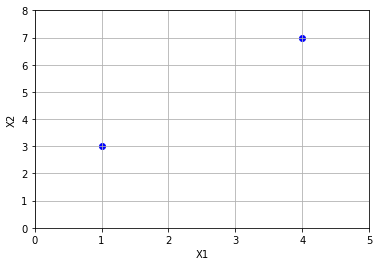
\includegraphics[width=0.3\textwidth]{1.1}
    \end{figure}
    \[\mu = \frac{1}{N}\sum_i x^{(i)} = (2.5, 5)\Rightarrow\text{after centering: }(-1.5, -2), (1.5, 2)\]
    \[\Rightarrow w = \text{norm}([1.5, 2]^{\top}) = [0.6, 0.8]^{\top}\]
    \item \[\mu = \frac{1}{N}\sum_i x^{(i)} = (4, 1)\Rightarrow\text{after centering: }(-2, -1), (-2, 1), (2, -1), (2, 1)\]
    \[\Rightarrow \Sigma = \frac{1}{N}XX^{\top} = 
    \begin{bmatrix}
        4 & 0\\
        0 & 1\\
    \end{bmatrix}\]
    \begin{figure} [!ht]
        \centering
        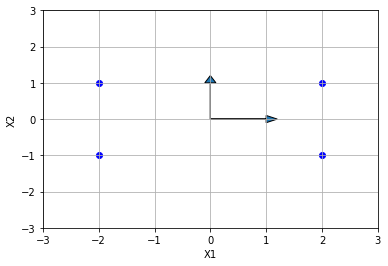
\includegraphics[width=0.3\textwidth]{1.2}
    \end{figure}
    \item The output of the program will be $12w_1^2 + 6w_2^2 + 20w_3^2 + 10w_4^2 = 12w_1^2 + 6w_2^2 + 20(1-w_1^2-w_2^2-w_4^2) + 10w_4^2 = 20 - 8w_1^2 - 14w_2^2 - 10w_4^2$. Therefore, eventually we have $w_1 = w_2 = w_4 = 0$ and thus $w = [0, 0, 1, 0]^{\top}$. The optimal value will be 20.
\end{enumerate}
\newpage

\section{Basics in Information Theory: 7pts}
\begin{enumerate}
    \item \[\Pr(X'=x) = \Pr(B=1)\cdot P(x) + \Pr(B=0)\cdot Q(x) = \lambda P(x) + (1-\lambda) Q(x)\]
    \item \[I(X';B) = H(X') - H(X'|B)\]
    \[= -\sum_x \Pr(X'=x)\log\Pr(X'=x)\] 
    \[+\lambda\sum_{x}\Pr(X'=x|B=1)\log\Pr(X'=x|B=1)\]
    \[+(1-\lambda)\sum_{x}\Pr(X'=x|B=0)\log\Pr(X'=x|B=0)\]

    \[= -\sum_x\left[\lambda P(x) + (1-\lambda) Q(x)\right]\log\left[\lambda P(x) + (1-\lambda) Q(x)\right]\]
    \[+\lambda\sum_{x}P(x)\log P(x) + (1-\lambda)\sum_{x}Q(x)\log Q(x)\]

    \[= \lambda\sum_{x} P(x)\left[\log P(x) - \log(\lambda P(x) + (1-\lambda) Q(x))\right]\]
    \[+ (1-\lambda)\sum_{x} Q(x)\left[\log Q(x) - \log(\lambda P(x) + (1-\lambda) Q(x))\right]\]

    \[= \lambda D_{KL}(P||\lambda P + (1-\lambda)Q) + (1-\lambda)D_{KL}(Q||\lambda P + (1-\lambda)Q)\]
    \[= D_\lambda(P||Q)\]
\end{enumerate}
\newpage

\section{k-Means with Soft Assignments: 10pts}
In all problems below, $A\cdot\textbf{1}_K = \textbf{1}_n$ stands true.
\begin{enumerate}
    \item It's equivalent to prove that for arbitrary $i\in\{1,\ldots,n\}$, we have:
    \[\min_{\mu_1,\mu_2,\ldots,\mu_K}\min_{A_i\in[0,1]^K}\sum_{k=1}^{K}A_{ik}\|x^{(i)} - \mu_k\|_2^2 \leq \min_{\mu_1,\mu_2,\ldots,\mu_K}\min_{A_i\in\{0,1\}^K}\sum_{k=1}^{K}A_{ik}\|x^{(i)} - \mu_k\|_2^2\]
    which is natural since $\{0,1\}^{K}$ is a subset of $[0,1]^{K}$, and thus the domain of $A_{ik}$ on LHS contains that on RHS. The equality will be reach if there is no value in $[0,1]\backslash\{0,1\}$ leading to a smaller outcome, otherwise there will be some $A_{ik}\in (0,1)$ making LHS smaller than RHS.
    \item Still, It's equivalent to prove that for arbitrary $i\in\{1,\ldots,n\}$, we have:
    \[\min_{\mu_1,\mu_2,\ldots,\mu_K}\min_{A_i\in[0,1]^K}\sum_{k=1}^{K}A_{ik}\|x^{(i)} - \mu_k\|_2^2 \geq \min_{\mu_1,\mu_2,\ldots,\mu_K}\min_{A_i\in\{0,1\}^K}\sum_{k=1}^{K}A_{ik}\|x^{(i)} - \mu_k\|_2^2\]
    Since $\|x^{(i)}-\mu_k\|^2_2 \geq \min_l\|x^{(i)} - \mu_l\|^2_2$, we have:
    \[\min_{\mu_1,\mu_2,\ldots,\mu_K}\min_{A_i\in[0,1]^K}\sum_{k=1}^{K}A_{ik}\|x^{(i)} - \mu_k\|_2^2 \geq \min_{\mu_1,\mu_2,\ldots,\mu_K}\min_{A_i\in[0,1]^K}\min_{l\in{1,\ldots,K}}\sum_{k=1}^{K}A_{ik}\|x^{(i)} - \mu_l\|_2^2\]
    Meanwhile:
    \[\min_{\mu_1,\mu_2,\ldots,\mu_K}\min_{A_i\in[0,1]^K}\min_{l\in{1,\ldots,K}}\sum_{k=1}^{K}A_{ik}\|x^{(i)} - \mu_l\|_2^2 = \min_{\mu_1,\mu_2,\ldots,\mu_K}\min_{A_i\in[0,1]^K}\min_{l\in{1,\ldots,K}}\|x^{(i)} - \mu_l\|_2^2\sum_{k=1}^{K}A_{ik}\]
    \[= \min_{\mu_1,\mu_2,\ldots,\mu_K}\min_{l\in{1,\ldots,K}}\|x^{(i)} - \mu_l\|_2^2\] 
    \[= \min_{\mu_1,\mu_2,\ldots,\mu_K}\min_{A_i\in\{0,1\}^K}\sum_{k=1}^{K}A_{ik}\|x^{(i)} - \mu_k\|_2^2,\;A\cdot\textbf{1}_K = \textbf{1}_n,\;\text{according to Eq. 2.}\]
    \item Since it's proved that LHS larger or equal and smaller or equal to RHS simultaneously, we have LHS equals to RHS, that is, the soft assignment gives the same outcome as the hard assignment. Nevertheless, in the last problem we showed that the optimal problem with $A\in [1,0]^{n\times K}$ will lead to $A\in \{1,0\}^{n\times K}$. Therefore, the problem in Eq. 3 corresponds to exactly the problem in Eq. 2
\end{enumerate}
\newpage

\section{Bernoulli Mixture Model: 18pt}
\begin{enumerate}
    \item \[\Pr(x^{(i)}|z_i,\mu) = \sum_{k=1}^{K}\left(z_{ik}\cdot\prod_{j=1}^{d}\mu_k^{x_j^{(i)}}(1-\mu_k)^{(1-x_j^{(i)})}\right)\] 
    % \[= \sum_{\textbf{z}_{i}}\prod_{k=1}^{K}\left(\prod_{j=1}^{d}\mu_k^{x_j^{(i)}}(1-\mu_k)^{(1-x_j^{(i)})}\right)^{z_{ik}} \cdot \pi_k^{z_ik}\]
    \[\Pr(z_i|\pi) = \prod_{k=1}^{K}\pi_k^{z_{ik}}\]
    \[\Rightarrow\log\Pr(x^{(i)},z_i|\pi,\mu) = \log\Pr(x^{(i)}|z_i,\mu)\Pr(z_i|\pi)\]
    \[= \log \sum_{k=1}^{K}\left(z_{ik}\cdot\prod_{j=1}^{d}\mu_k^{x_j^{(i)}}(1-\mu_k)^{(1-x_j^{(i)})}\right)\prod_{k=1}^{K}\pi_k^{z_{ik}}\]

    \item \[z_{ik}^{new} = \Pr(z_{ik}=1|x^{(i)}) = \frac{\Pr(z_{ik}=1)\Pr(x^{(i)}|z_{ik}=1)}{\sum_{\hat{k}=1}^{K}\Pr(z_{i\hat{k}}=1)\Pr(x^{(i)}|z_{i\hat{k}}=1)}\]
    \[= \frac{\displaystyle\pi_{k}\prod_{j=1}^{d}\mu_k^{x_j^{(i)}}(1-\mu_k)^{(1-x_j^{(i)})}}{\displaystyle\sum_{\hat{k}=1}^{K}\left(\pi_{\hat{k}}\prod_{j=1}^{d}\mu_{\hat{k}}^{x_j^{(i)}}(1-\mu_{\hat{k}})^{(1-x_j^{(i)})}\right)}\]

    \item The log likelihood $\log\Pr(x^{(i)},z_i|\pi,\mu)$ can be written in form:
    \[\log\prod_{j=1}^{d}\mu_{k'}^{x_j^{(i)}}(1-\mu_{k'})^{(1-x_j^{(i)})} + \log\pi_{k'}\]
    in which $k_{ik'} = 1$. For $\frac{\partial}{\partial\mu_k}$, say there are $j$ of number $m$ such that $x^{(i)}_j = 1$, then we have:
    \[\frac{\partial}{\partial\mu_{k'}}: \frac{\left(\mu_{k'}^{m}(1-\mu_{k'})^{d-m}\right)'}{\mu_{k'}^{m}(1-\mu_{k'})^{d-m}} = \frac{m-d\mu_{k'}}{\mu_{k'}(1-\mu_{k'})} = 0\]
    in which $m = \sum_{j=1}^{d}x_j^{(i)}$.
    \newpage
    Hence, we have:
    \[\frac{\partial}{\partial\mu_k}: -\sum_{i=1}^{n}z_{ik}^{new}\left(d\mu_k - \sum_{j=1}^{d}x_j^{(i)}\right) = 0\]
    \[\Rightarrow \mu_{k}^{new} = \frac{1}{N_k}\sum_{i=1}^{n}\left(z_{ik}^{new}\cdot\frac{\sum_{j=1}^{d}x^{(i)}_{j}}{d}\right)\]
    \[= \frac{1}{N_k}\sum_{i=1}^{n}\left(\frac{\pi_{k}\prod_{j=1}^{d}\mu_k^{x_j^{(i)}}(1-\mu_k)^{(1-x_j^{(i)})}}{\sum_{\hat{k}=1}^{K}\left(\pi_{\hat{k}}\prod_{j=1}^{d}\mu_{\hat{k}}^{x_j^{(i)}}(1-\mu_{\hat{k}})^{(1-x_j^{(i)})}\right)}\cdot\frac{\sum_{j=1}^{d}x^{(i)}_{j}}{d}\right)\]
    in which $N_k = \sum_{i=1}^{n}z_{ik}^{new}$.
    For $\frac{\partial}{\partial\pi_k}$, we have:
    \[\frac{\partial}{\partial\pi_{k}}: \sum_{i=1}^{n}\frac{\prod_{j=1}^{d}\mu_k^{x_j^{(i)}}(1-\mu_k)^{(1-x_j^{(i)})}}{\sum_{\hat{k}=1}^{K}\left(\pi_{\hat{k}}\prod_{j=1}^{d}\mu_{\hat{k}}^{x_j^{(i)}}(1-\mu_{\hat{k}})^{(1-x_j^{(i)})}\right)} + \lambda = 0\]
    in which $\lambda$ is the Lagrangian multiplier for the constraint $\sum_{k=1}^{K}\pi_k = 1$.
    \[\Rightarrow\pi_{k}^{new} = \frac{N_k}{n}\]
\end{enumerate}
\newpage

\section{Variational Autoencoder (VAE): 19pts}
\begin{enumerate}
    \item[3.]
    \begin{enumerate}
        \item[(a)] Empirical risks:
        \begin{figure}[h]
            \centering
            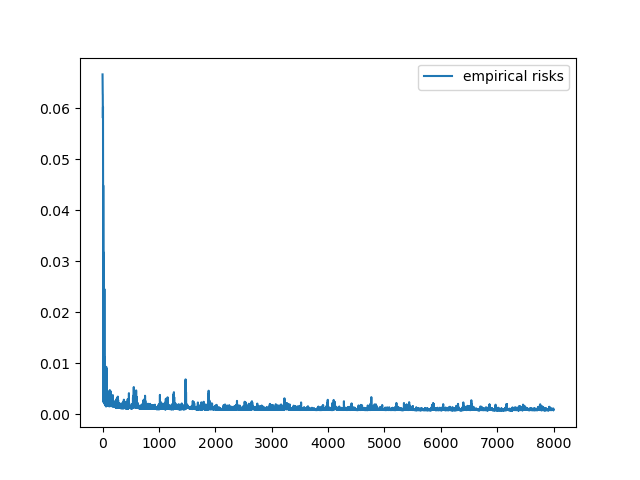
\includegraphics[width=0.6\textwidth]{5.3a}
        \end{figure}
        \item[(b)] Data points along with approximations:
        \begin{figure}[h]
            \centering
            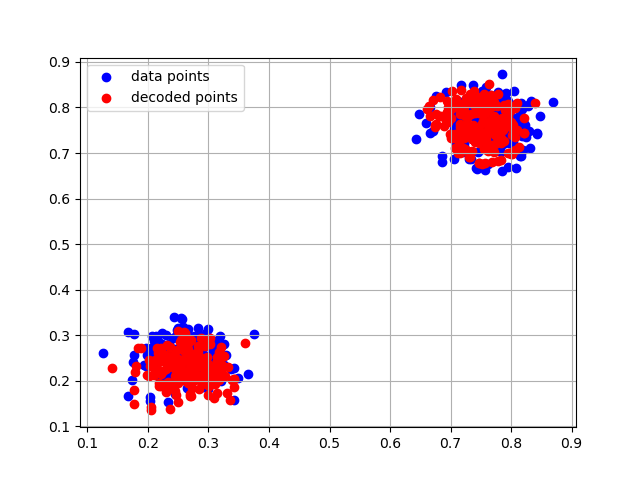
\includegraphics[width=0.6\textwidth]{5.3b}
        \end{figure}
        \newpage
        \item[(c)] Data points along with approximations and generated points according to uniform distribution:
        \begin{figure}[h]
            \centering
            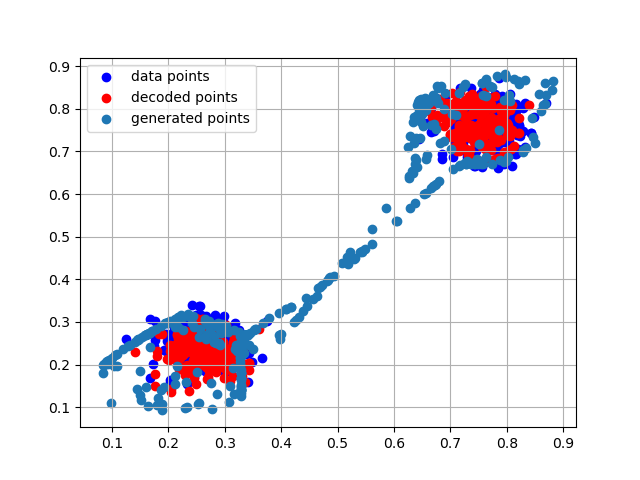
\includegraphics[width=0.6\textwidth]{5.3c}
        \end{figure}
    \end{enumerate}
\end{enumerate}

\end{document}